\subsection{Gravitational Waves from Collision of Neutron Stars}

\subsubsection{The First BNS Merger Detection: GW170817}
 
The stage was set, LIGO's second observation run 02 was coming to a close. When a week was left, on 17th august 2017, the LIGO and Virgo observatory came online and detected a Gravitational Wave (GW170817). Two seconds after the LIGO and Virgo GW detection, the fermi satellite detected a burst of gamma ray radiation (GRB170817A). So loud, you can see it by eye (SNR=32.4). This alerted telescopes and satellites all over the world, which gave the beginning to the most studied astronomical event (-1225 days).  
 
\subsubsection{The origin of the GW170817}
 
$135$ Million years ago, two neutron stars were spiralling faster and faster, stretching and squeezing space-time which created distortions in the fabric, which is gravitational waves. As soon as they reached the distance between Atlanta and Nash-field, they started merging. When they merged it produced a huge explosion of gamma ray radiation. In the last $\frac{1}{10}^{th}$ of a second, the energy released by these stars were 50 times greater than anything else in the universe. Theses waves reached earth after travelling billions of light years in the speed of light. We interpret the component masses of these stars to be between $0.86M\textsubscript{\(\odot\)}$ and $2.26\textsubscript{\(\odot\)}$, in agreement with masses of neutron stars. The closest and most precisely calculated gravitational wave signal yet. This gravitational wave signalises loudest yet observed, with a combined signal to noise ratio of 32.4. After the study conducted, it led to look at an area of 28 $\text{deg}^{2}$.\\
Which led to the discovery of its home NGC 4993. Normally we believe that if neutron stars merged and formed heavier neutron stars which spins rapidly and generates a very strong magnetic field. But it lead to the formation of lowest mass black hole ever found. 
 
\subsubsection{The dynamics of neutron-star binaries and collision}

The initial coordinate separation between the maxima in the rest-mass density is 45 km. The neutron stars inspiral with increasing angular velocity, which deforms each of them tidally. This increases the inspiral rate as it depends on total angular momentum of the system. 

\begin{figure}[h]
    \centering
    \subfloat[]{{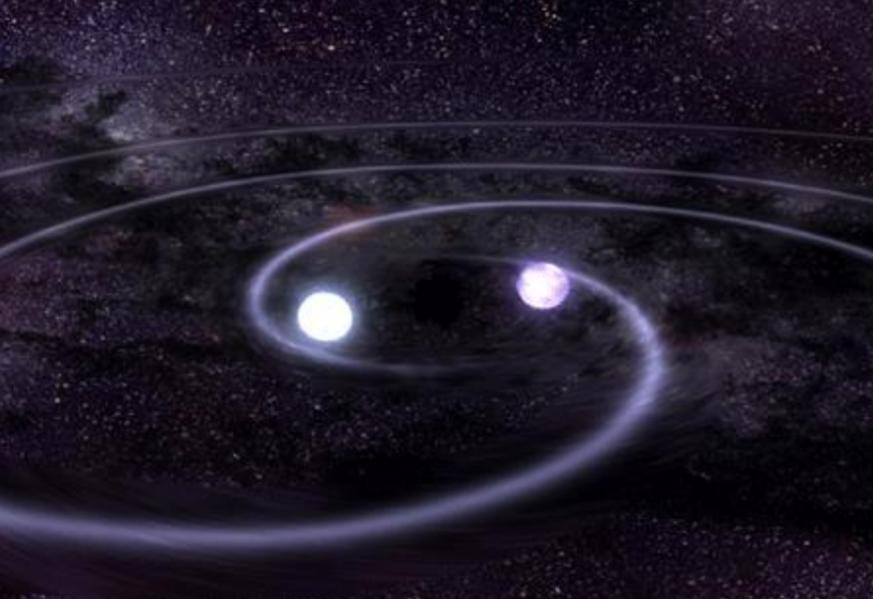
\includegraphics[scale=0.2]{images.tex/INSPIRAL.jpg}}}
    \qquad
    \subfloat[]{{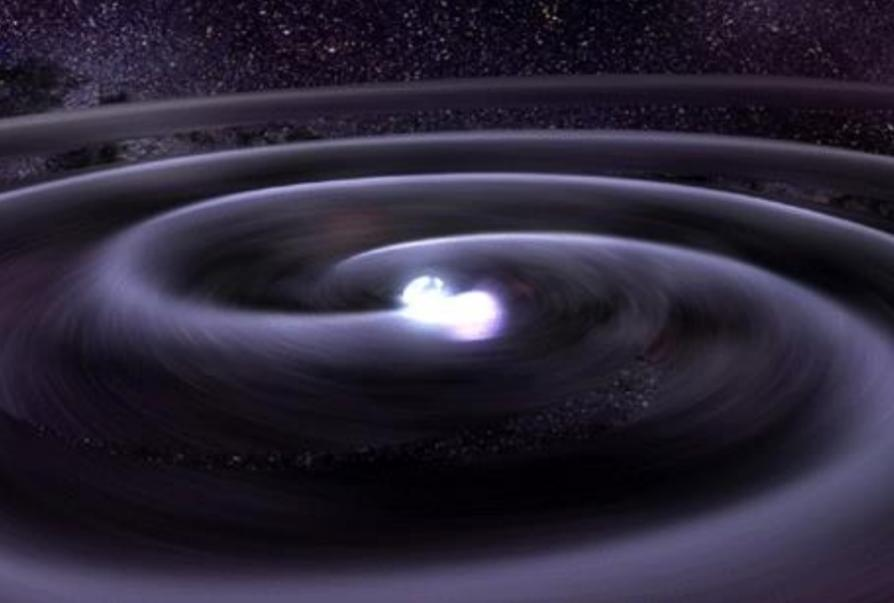
\includegraphics[scale=0.2]{images.tex/MERGER.jpeg}}}
    \caption{(a) Neutron stars in inspiral mechanism. (b) Neutron stars in merger phase.\\ Source:- \href{https://youtu.be/y8VDwGi0r0E}{Neutron Star Merger in YouTube}}
\end{figure}

\noindent
During the merger, when regions of the neutron stars with density less than their maximum density come into contact, the tangential components of the velocity exhibit a discontinuity. This can develop an instability called the Kelvin-Helmholtz instability, which leads to the overall amplification of the magnetic field. Such high magnetic fields are seen in magnetars and short hard gamma-ray bursts, which are the consequences of the neutron star collision.

After the merger, the cores of the two neutron stars combine into one and the central rest-mass density starts increasing. The maximum rest-mass density then increases exponentially, and the object collapses to a rotating black hole. This was seen in the detection of gravitational wave- GW170817.

\begin{figure}[h]
    \centering
    \subfloat[]{{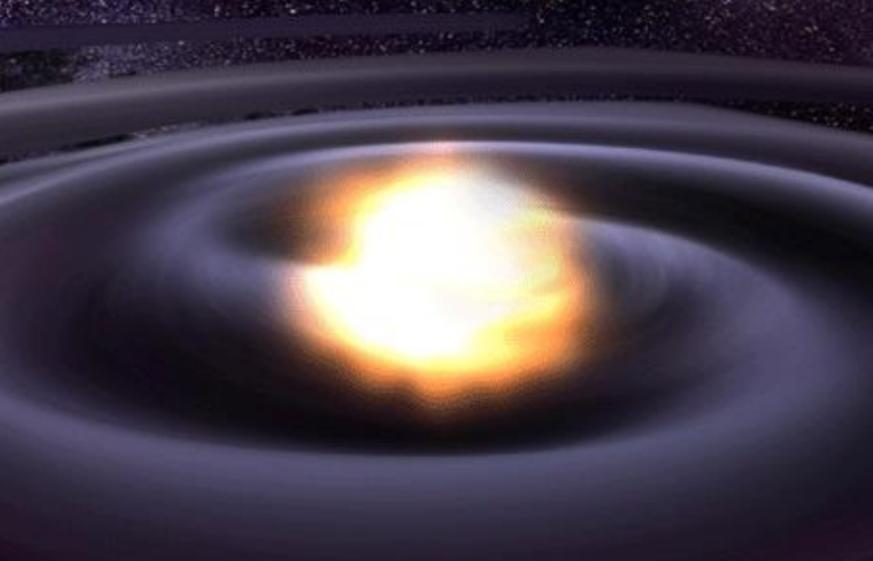
\includegraphics[scale=0.235]{images.tex/MERGER2.jpeg}}}
    \qquad
    \subfloat[]{{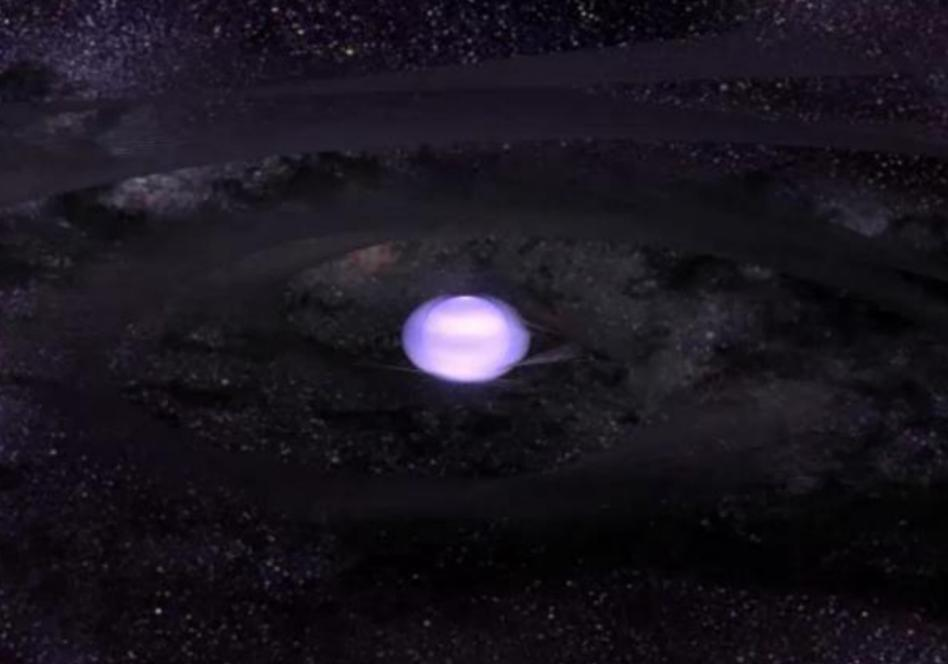
\includegraphics[scale=0.1992]{images.tex/RINGDOWN.jpeg}}}
    \caption{(a) Neutron stars after merging. (b) Neutron stars in ring-down phase. \\ Source :- \href{https://youtu.be/y8VDwGi0r0E}{Neutron Star Merger in YouTube}} 
\end{figure}

In accordance with the dynamics of the neutron-star binaries, during the inspiral, gravitational wave forms increase in amplitude and in frequency. 
The wave forms after the merger have more variation and finally they try to become a stable body, thus even the emission of gravitational wave decreases exponentially with time. Hence, in many cases, the wave forms after the merger mostly terminate during the ring down. The ring down signal for black holes formed in binary neutron star mergers is at frequencies of the order of kHz and cannot be detected by the present detectors so easily. The post-merger signal is at lower frequencies than the ring down. Here we have a picture of waveform of gravitational waves emitted from a neutron stars merger. and axes represents strain in space vs time in various modes. Initially the strain which signifies the frequency of waves, and it's amplitude is small which increases slowly with time, reach a peak in merger phase, then abruptly become zero during ring down phase.

\begin{figure}[h]
    \centering
    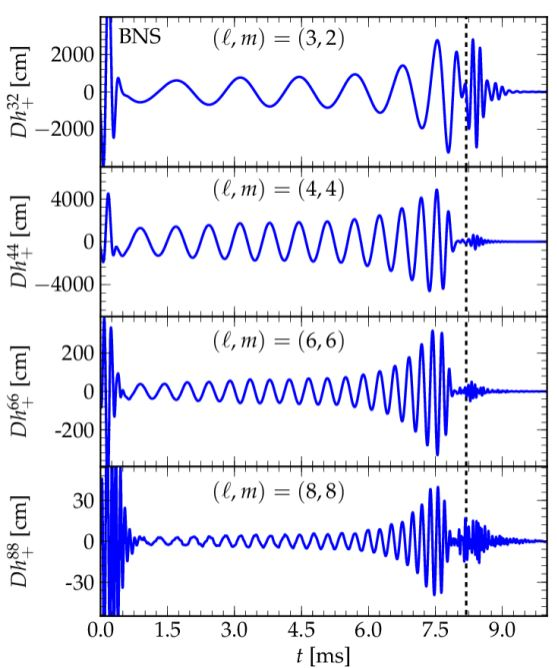
\includegraphics[scale=0.74]{images.tex/WAVEFORM.jpeg}
    \caption{Gravitational Waveform by Neutron star collision. Source :- \href{https://www.researchgate.net/figure/Binary-neutron-stars-GW-modes-m-3-2-4-4-6-6-8-8-of-polarization_fig13_233846764}{Research Gate}}
\end{figure}

\pagebreak
